\documentclass[12pt,a3paper]{article}
\usepackage[utf8]{inputenc}
\usepackage[spanish,es-sloppy]{babel}
\usepackage{amsmath}
\usepackage{amsfonts}
\usepackage{amssymb}
\usepackage{graphicx}
\usepackage{here}
\usepackage[left=1.8cm,right=1.8cm,top=1.5cm,bottom=1.5cm]{geometry}
\usepackage{verbments}
%\definecolor{fondo1}{rgb}{0.9764, 0.9764, 0.9762}
%\definecolor{fondo2}{rgb}{0.1647, 0.4980, 0.7}
\definecolor{fondo1}{rgb}{0.88, 0.88, 0.88}
\definecolor{fondo2}{rgb}{0.15, 0.15, 0.5}
\author{Josue Huaroto Villavicencio - 20174070I}
\title{1$^{\circ}$ Práctica de Cálculo por Elementos Finitos - MC516}
\date{Sección: E}
\begin{document}
\fvset{frame=bottomline, framerule=0.02cm,numbers=left, numbersep=8pt}
\plset{language=python,texcl=true,listingnamefont=\sffamily\bfseries\color{white},captionbgcolor=fondo2, bgcolor=fondo1,listingname=\textbf{Código}, captionfont=\sffamily\color{white},fontsize=\small}
\maketitle
%\tableofcontents
\section{Diagrama de flujo}
\begin{figure}[H]
\begin{center}
\includegraphics[scale=0.65]{flujo.png}
\end{center}
\end{figure}
\section{Optimizadores de rendimiento}
Para optimizar el código, se eligió reducir la complejidad computacional de la multiplicación de matrices y la complejidad del solucionador clásico de ecuaciones lineales.
\subsection{Algoritmo de Strassen}
Para mejorar la alta complejidad de la mutliplicación ingenua se utiliza el algoritmo de Strassen, la cual puede reducir la complejidad computacional al usar un enfoque Divide \& Conquer y reducir la cantidad de operaciones de una matriz a 7 en vez de 8; entonces la complejidad final se reduce de $\log_{2} 8$ a $\log_{2} 7$. $\mathcal{O}(n^{2.8})$.
\begin{pyglist}[language=python,caption={Multiplicación Rápida:\hspace{5pt} $\mathcal{O}(n^{\log_{2} 7})$},
style=pastie]
def FastMultiply(oldA,oldB):
    rows = oldA.shape[0]
    columns = oldB.shape[1]
    if(rows <=2 or columns<=2 or oldA.shape[1]<=2 or oldB.shape[0] <= 2):
        return np.matmul(oldA,oldB) 
    A = ModifyMatrix(oldA)
    B = ModifyMatrix(oldB)
    N1 = A.shape[0]
    N2 = A.shape[1]
    N3 = B.shape[0]
    N4 = B.shape[1]
    a = A[0:N1//2,0:N2//2]
    b = A[0:N1//2,N2//2:N2//2+N2//2]
    c = A[N1//2:N1//2+N1//2,0:N2//2]
    d = A[N1//2:N1//2+N1//2,N2//2:N2//2+N2//2]
    e = B[0:N3//2,0:N4//2]
    f = B[0:N3//2,N4//2:N4//2+N4//2]
    g = B[N3//2:N3//2+N3//2,0:N4//2]
    h = B[N3//2:N3//2+N3//2,N4//2:N4//2+N4//2]
    p1 = FastMultiply(a,(f-h))
    p3 = FastMultiply((c+d),e)
    p2 = FastMultiply((a+b),h)
    p4 = FastMultiply(d,(g-e))
    p5 = FastMultiply((a+d),(e+h))
    p6 = FastMultiply((b-d),(g+h))
    p7 = FastMultiply((a-c),(e+f))
    C = np.zeros((rows,columns))
    c11 = p5 + p4 - p2 + p6
    c12 = p1 + p2
    c21 = p3 + p4
    c22 = p1 + p5 - p3 - p7
    for i in range(0,N1//2):
        for j in range(0,N4//2):
            C[i][j] = c11[i][j]
            if(j + N4//2 < columns):
                C[i][j+N4//2] = c12[i][j]
            if(i + N1//2 < rows):
                C[i+N1//2][j] = c21[i][j]
                if(j + N4//2 < columns):
                    C[i+N1//2][j+N4//2] = c22[i][j]
    return C
\end{pyglist}
Sin embargo, la constante es demasiado alta. El algoritmo no es eficiente para tamaños pequeños, por debajo de 50 es más eficiente la multiplicación ingenua.
\subsection{Gradiente conjugado}
Una forma de resolver más rápido sistemas de ecuaciones lineales para matrices simétricas es utilizar el método del gradiente conjugado. La complejidad de la reducción de Cholesky o Gauss, o los métodos iterativos como los de Gauss-Seidel o Jacobi son poco eficientes para matrices grandes; el algoritmo de gradiente conjugado es capaz de reducir la complejidad de  $\mathcal{O}(n^3)$ a $\mathcal{O}(n^2)$. Dado a que la mayoría de problemas lineales en elementos finitos presentan matrices de rigidez simétricas es óptimo la elección de este método para acelerar las soluciones.
\begin{pyglist}[language=python,caption={Conjugate Gradient:\hspace{5pt} $\mathcal{O}(2n^2)$},style=pastie]
def conjugate_grad(A, b, x=None):
    n = b.shape[0]
    if not x:
        x = np.ones((n,1))
    r = np.dot(A, x) - b
    p = - r
    r_k_norm = FastMultiply(np.transpose(r), r)
    for i in range(2*n):
        Ap = np.dot(A, p)
        alpha = r_k_norm/FastMultiply(np.transpose(p), Ap)
        x += alpha * p
        r += alpha * Ap
        r_kplus1_norm = FastMultiply(np.transpose(r), r)
        beta = r_kplus1_norm/r_k_norm
        r_k_norm = r_kplus1_norm
        p = beta * p - r
    return x
\end{pyglist}
\section{Solucionador}
Para simplificar la sintaxis general de resolver un problema de elementos finitos que implique una solución directa y elementos barras se diseñó un código para separar tareas generales que permiten automatizar el código.
\subsection{Definición de condiciones}
Esta parte del código sirve para definir las condiciones de frontera como los soportes o fuerzas nodales.
\begin{pyglist}[language=python,caption={Condiciones de frontera},style=pastie]
NodesCondition = []
ForcesCondition = []
def UBoundaryCondition(nU,u,i):
    nU[i][0] = u
    NodesCondition.append(i)
def FBoundaryCondition(nF,f,i):
    nF[i][0] = f
    ForcesCondition.append(i)
\end{pyglist}
\subsection{Ensamble de matriz de rigidez}
Con los datos del problema se crea una matriz de rigidez simétricas ensamblada que se utilizará para resolver el problema.
\begin{pyglist}[language=python,caption={Ensamble de matriz de rigidez},style=pastie]
def AssemblyStiffness(nStiffnessMatrix,k,i,j):
    nStiffnessMatrix[i][i] += k
    nStiffnessMatrix[i][j] += -k
    nStiffnessMatrix[j][i] += -k
    nStiffnessMatrix[j][j] += k
def Initialize(nStiffnessMatrix,nU,nF):
    for i in range(0,NumberOfElement):
        AssemblyStiffness(nStiffnessMatrix,K[i][0],int(K[i][1]),int(K[i][2]))
\end{pyglist}
\subsection{Preparación de la matriz de rigidez}
Se elimina filas y columnas de la matriz de rigidez que permita despejar el sistema y dejar una forma equivalente a $\mathbf{A}x = \mathbf{B}$.
\begin{pyglist}[language=python,caption={Preparación de matriz de rigidez},style=pastie]
def PreSolvingStiffness(nStiffnessMatrix):
    nsize = Nodes-len(NodesCondition)
    newStiffness = np.zeros((nsize,nsize))
    contr = -1
    for i in range(0,Nodes):
        contc = -1
        flagr = False
        for k in range(0,len(NodesCondition)):
            if(i == NodesCondition[k]):
                flagr = True
                break
        if(flagr):
            continue
        contr += 1
        for j in range(0,Nodes):
            flagc = False
            for k in range(0,len(NodesCondition)):
                if(j == NodesCondition[k]):
                    flagc = True
                    break
            if(flagc):
                continue
            contc += 1
            newStiffness[contr][contc] = nStiffnessMatrix[i][j]
    return newStiffness
\end{pyglist}
\subsection{Pre-solver de la matriz de fuerzas}
\begin{pyglist}[language=python,caption={Pre-solver de la matriz de fuerzas},style=pastie]
def PreSolvingF(nF,nS,nU):
    nsize = Nodes-len(NodesCondition)
    newF = np.zeros(nsize).reshape(nsize,1)
    contr = -1
    for i in range(0,Nodes):
        flagr = False
        for k in range(0,len(NodesCondition)):
            if(i == NodesCondition[k]):
                flagr = True
                break
        if(flagr):
            for k in range(0,Nodes):
                nF[k][0] = nF[k][0]-nS[k][i]*nU[i][0]
            continue
    for i in range(0,Nodes):
        flagr = False
        for k in range(0,len(NodesCondition)):
            if(i == NodesCondition[k]):
                flagr = True
                break
        if(flagr):
            continue
        contr += 1
        newF[contr][0] = nF[i][0]  
    return newF
\end{pyglist}
\subsection{Solver}
Se utiliza el método del gradiente conjugado para resolver el sistema despejado, finalmente; se reemplaza en las matrices originales y se usa el algoritmo de Strassen para armar la solución final.
\begin{pyglist}[language=python,caption={Solver},style=pastie]
def Solve(nStiffnessMatrix,nU,nF):
    newStiffness = PreSolvingStiffness(nStiffnessMatrix)
    newF = PreSolvingF(nF,nStiffnessMatrix,nU)
    u = conjugate_grad(newStiffness,newF)    
    contr = -1
    for i in range(0,Nodes):
        flagr = False
        for k in range(0,len(NodesCondition)):
            if(i == NodesCondition[k]):
                flagr = True
                break
        if(flagr):
            continue
        contr += 1
        nU[i][0] = u[contr][0]
    nnF = FastMultiply(StiffnessMatrix,nU)
    return nU,nnF
\end{pyglist}
\section{Ejecución del código}
Las condiciones del problema se establecen en esta sección del código, aquí se definen las condiciones de frontera, características geométricas y físicas y fuerzas aplicadas; así como la cantidad de nodos y elementos para la solución.
\begin{pyglist}[language=python,caption={Condiciones del problema},style=pastie]
NodesCondition = []
Nodes = 4
Nodes = 2*Nodes+1
E = 2*1e5 #MPA
L = 1500 #mm
b0 = 1000 #mm
bf = 0 #mm
e = 120 #mm
P = 50000 #N
y = 0.0784532e-3 #N/mm3
A = []
K = []
for i in range(0,Nodes):
    b = b0-i*((b0-bf)/(Nodes-1))
	nb = b-(b0-bf)/(Nodes-1)    
    A.append((b+nb)*e/2)
for i in range(0,Nodes-1):
    K.append([E*A[i]/(L/(Nodes-1)),i,i+1])
NumberOfElement = len(K)
StiffnessMatrix = np.zeros((Nodes,Nodes))
U = np.zeros(Nodes).reshape(Nodes,1)
F = np.zeros(Nodes).reshape(Nodes,1)
Initialize(StiffnessMatrix,U,F)
UBoundaryCondition(U,0,0)
for i in range(1,Nodes):
    if(i%2 == 1):
        W = y*(A[i]+A[i-1])*(L/(Nodes-1))
        FBoundaryCondition(F,W,i)
    else:
        FBoundaryCondition(F,0,i)     
if((NumberOfElement//2)%2 == 1):
    W = y*(A[NumberOfElement//2]+A[NumberOfElement//2-1])*(L/(Nodes-1))
    FBoundaryCondition(F,P+W,NumberOfElement//2)
else:
    FBoundaryCondition(F,P,NumberOfElement//2)
U,F=Solve(StiffnessMatrix,U,F)
print("Stiffness Matrix:\n",StiffnessMatrix,'\n')
print("Displacements:\n",U,'\n')
print("Forces:\n",F)
\end{pyglist}
La gráfica de la fuerza sobre los nodos se muestra a continuación, se puede apreciar que existen unos pequeños picos para los primeros elementos; esto es porque corresponden al peso, luego para la mitad se ve un pico más pronunciado que corresponde a la carga central; luego para los últimos elementos se observa que el peso es prácticamente insignificante para la parte final de la placa triangular en comparación con la base.
\begin{figure}[H]
\begin{center}
\includegraphics[scale=0.51]{forze20.pdf}
\includegraphics[scale=0.51]{def30.pdf}
\caption{Fuerza y desplazamiento para 30 nodos}
\end{center}
\end{figure}
La gráfica de la deformación muestra un comportamiento lineal hasta el nodo donde se aplica la carga externa; para luego cambiar de pendiente.
\section{Resultados del problema}
El problema se modela de la siguiente forma: dos elementos se representan con 3 nodos, y el nodo central es utilizado para colocar el peso de los dos elementos; de esta forma el peso de los dos elementos es colocado en el nodo medio como una carga externa única para ese nodo; dado que dos elementos consecutivos se diferencian en un volumen muy pequeño el nodo medio representa al centro de gravedad de los dos elementos juntos. Con esta formulación se duplica la cantidad de elementos pero es posible modelar la placa como una unión simple de elementos barra.
\begin{figure}[H]
\begin{center}
\includegraphics[scale=0.58]{PROB.png}
\includegraphics[scale=0.34]{noc.png}
\caption{Matriz de rigidez, fuerzas, desplazamientos y esfuerzos para 4 elementos}
\end{center}
\end{figure}
La fuerza de reacción en el apoyo corresponde a la fuerza en el nodo 0: \fbox{-57060.788 N}
\begin{figure}[H]
\begin{center}
\includegraphics[scale=0.5]{HDEFOR.pdf}
\includegraphics[scale=0.5]{waits.pdf}
\caption{Distribución de deformaciones y esfuerzos considerando solo el peso de la placa}
\end{center}
\end{figure}
\begin{figure}[H]
\begin{center}
\includegraphics[scale=0.5]{gg.pdf}
\includegraphics[scale=0.5]{Heatmap.pdf}
\caption{Distribución de deformaciones y esfuerzos de la placa}
\end{center}
\end{figure}
\section{Problema generalizado para $n$ nodos}
\begin{figure}[H]
\begin{center}
\includegraphics[scale=0.72]{Stiffness.png}
\includegraphics[scale=0.51]{fordis.png}
\caption{Matriz de rigidez, fuerzas y desplazamientos para 11 nodos}
\end{center}
\end{figure}
Para incrementar la precisión de los resultados se elige utilizar una mayor cantidad de elementos, debido a las limitaciones de memoria, usaremos solo 2000 elementos; el cual se logra ejecutar en python en alrededor de 1 segundo.
\begin{figure}[H]
\begin{center}
\includegraphics[scale=0.32]{data.png}
\includegraphics[scale=0.58]{21.pdf}
\includegraphics[scale=0.58]{22.pdf}
\caption{Deformaciones, fuerzas y esfuerzos para 2000 elementos - Discretización con 20 elementos}
\end{center}
\end{figure}
\section{Verificación de resultados}
Para la verificación de los cálculos se utilizó el software Ansys.
%\begin{figure}[H]
%\begin{center}
%\includegraphics[scale=0.4]{mesh.png}
%\caption{Mallado}
%\end{center}
%\end{figure}
\begin{figure}[H]
\begin{center}
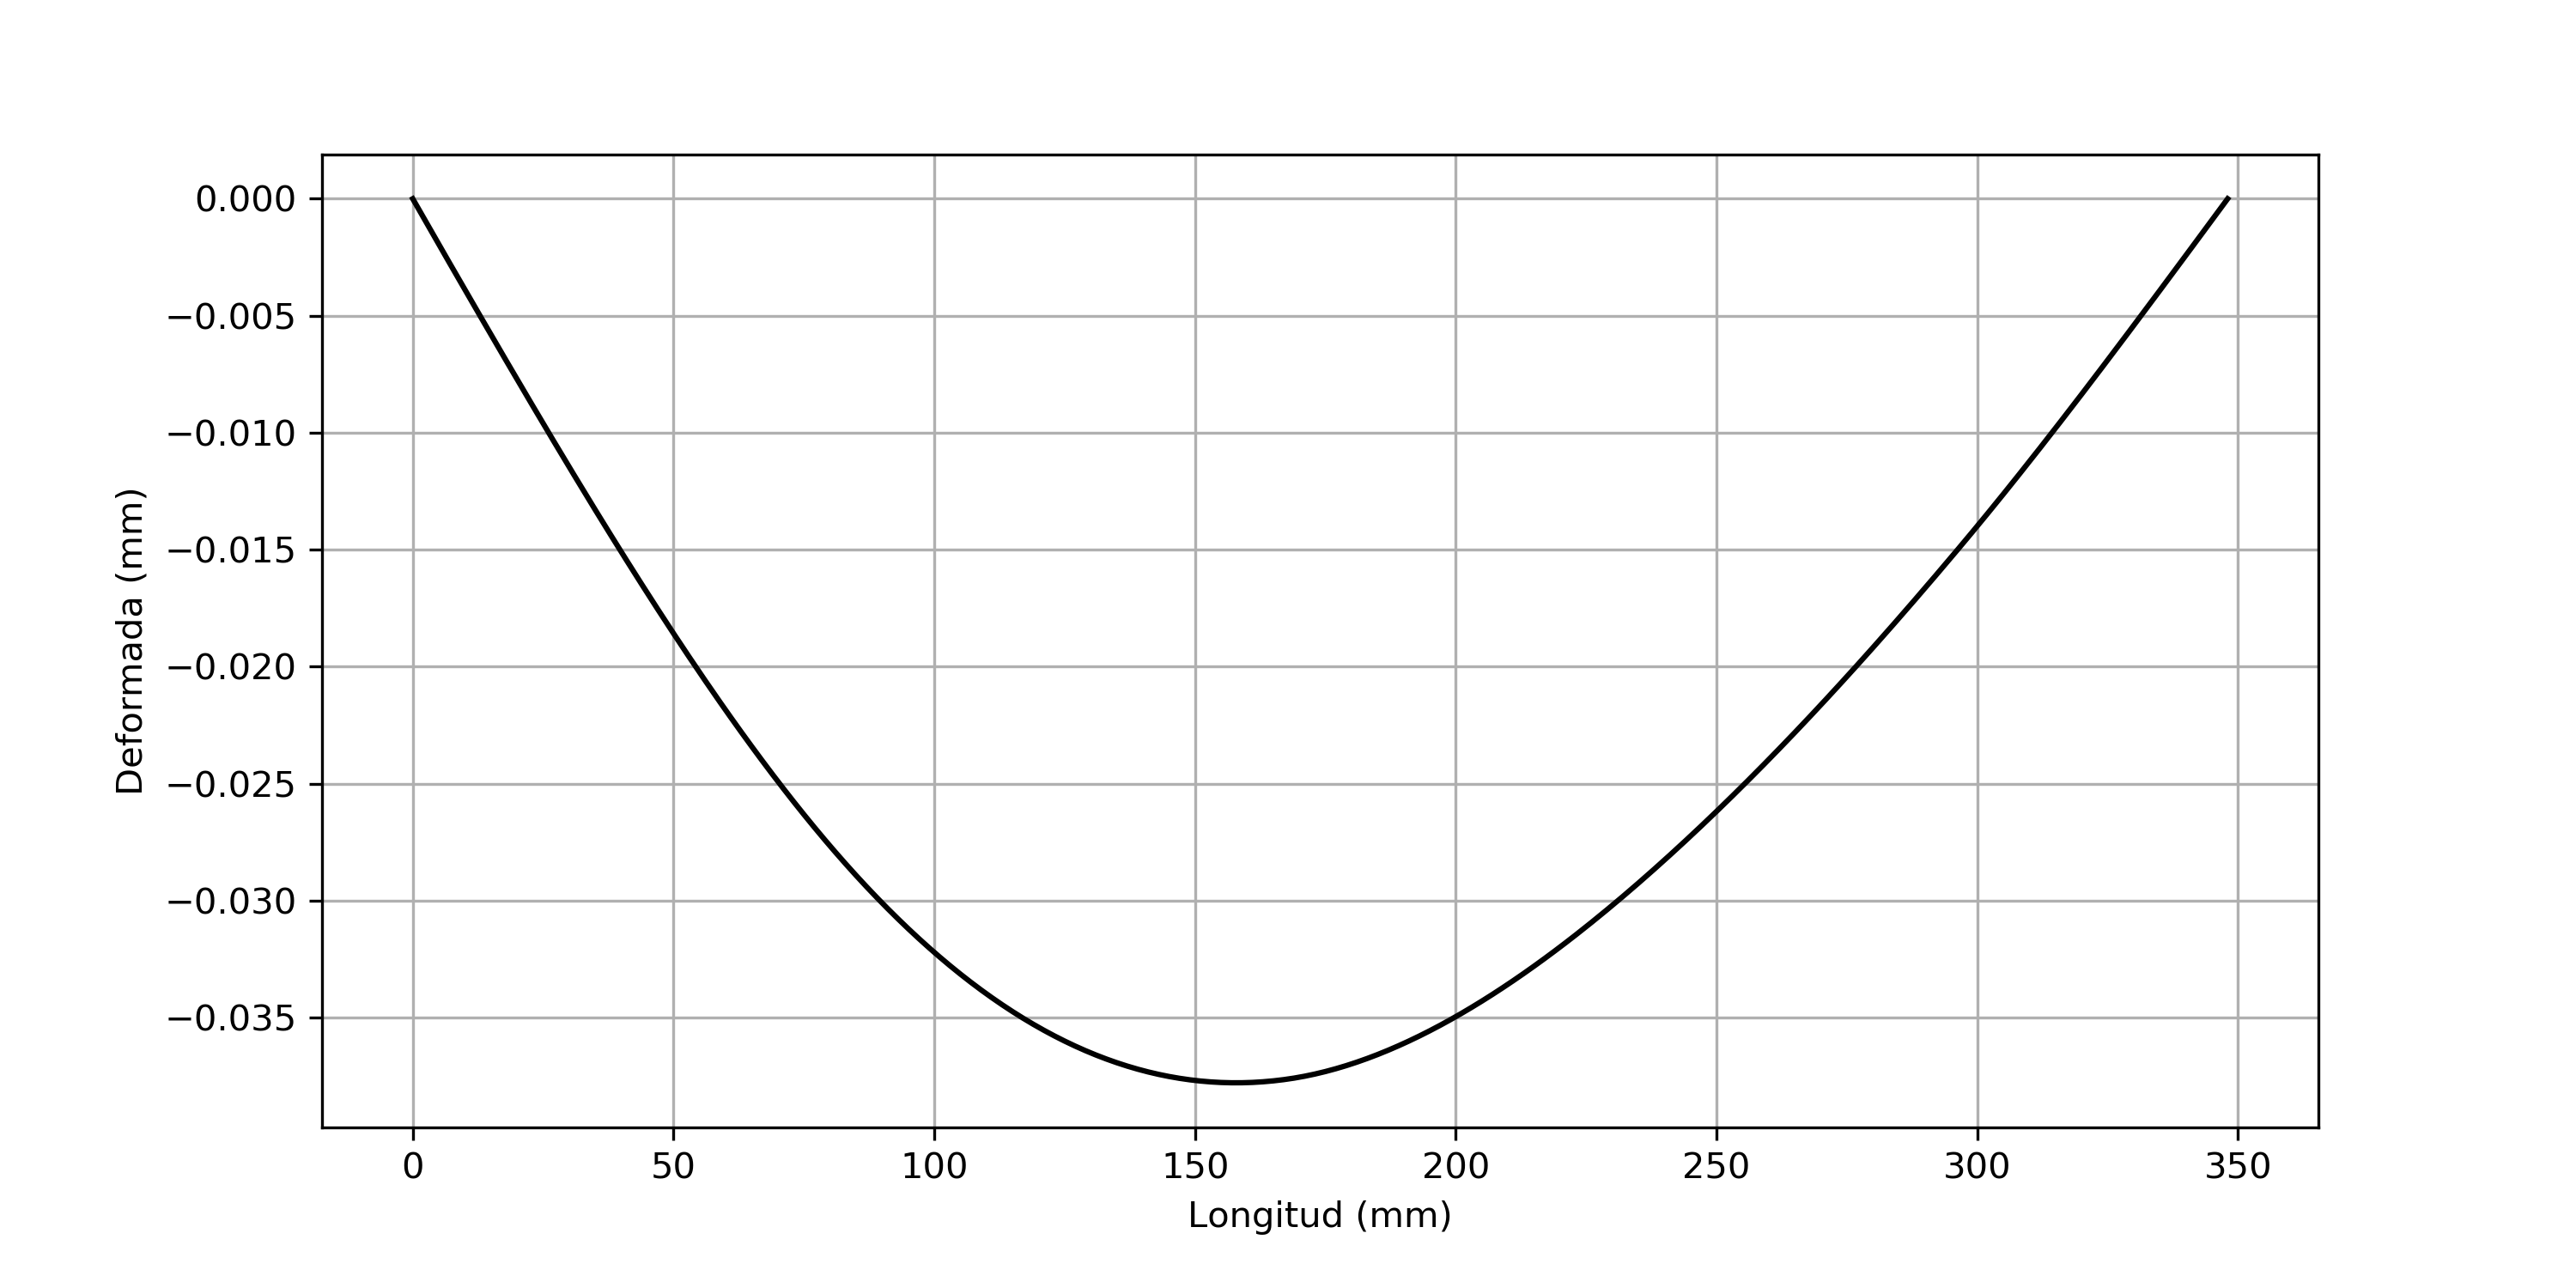
\includegraphics[scale=0.45]{def.png}
\includegraphics[scale=0.45]{stress.png}
\caption{Deformaciones y esfuerzos}
\end{center}
\end{figure}
\section{Conclusiones}
\begin{enumerate}
\item Es posible despreciar el peso de la placa porque es muy pequeña la fuerza en comparación con la carga central.
\item La cantidad de elementos para la convergencia de la solución es de aproximadamente 50.
\item Incrementar la cantidad de elementos puede parecer una estrategia viable para mejorar la convergencia de la solución; pero al incrementar la cantidad de elementos sus dimensiones son menos aceptables para ser tratado como un elemento barra por sus medidas geométricas.
\item Se sugiere usar un elemento de mayor dimensión para poder modelar de forma más precisa los esfuerzos y deformaciones.
\item La estrategia de ubicar el peso en un nodo medio entre dos elementos es una estrategia que permite acercarnos a la respuesta cuando es necesario ubicar cargas sobre un continuo.
\item El modelado hecho con elemento barra cumple los criterios debido a que la deformación de la placa en otros ejes es despreciable y se considera únicamente deformación en una dirección.
\item El algoritmo de Strassen junto con el algoritmo del gradiente conjugado son capaces de acelerar hasta 10 veces el código para matrices de gran tamaño.
\item El tiempo esperado por solución es de a lo mucho 10 segundos para 10000 elementos.
\item La implementación del código en Python es lo suficientemente rápido y corto para realizarse en unos pocos minutos.
\item La implementación del código en MatLab es más simple y corta pero demasiado lenta; tardando varios minutos para ejecutar 1000 elementos.
\end{enumerate}
\begin{center}
\begin{tabular}{|c|c|}
\hline 
Lenguaje/Cantidad de elementos & Tiempo de ejecución (s) \\ 
\hline 
C++/1000 & 0.3 \\ 
\hline 
Python/1000 & 4.2 \\ 
\hline 
MatLab/1000 & 357.7 \\ 
\hline 
\end{tabular} 
\end{center}
\section{Agradecimientos}
El presente trabajo me permitió desarrollar y aplicar gran parte de mi conocimiento en el desarrollo y optimización de algoritmos; como programador competitivo constantemente intento optimizar mis algoritmos lo más posible y en este caso no fue la excepción. El código permite una generalización para cualquier problema que pueda ser modelado con barras con tan solo unas pocas modificaciones en la parte final del código; como tal puede tratarse como un solver eficiente para elementos finitos. Así mismo, espero que este sea uno de las primeras implementaciones que realice para poder tener un repertorio más amplio de elementos en el futuro.\\
El trabajo inicial fue muy simple de realizar, pero en busca de optimizar el código me vi en la necesidad de recurrir al algoritmo de Strassen; sin embargo, aún necesitaba de un solver que utilizara de forma eficiente las multiplicaciones hechas por el algoritmo; el método del gradiente conjugado trabaja mejor que Gauss-Seidel para matrices simétricas y grandes; por lo que fue la elección para resolver el sistema.\\
El código en Python era lo suficientemente rápido como para computar más de 2000 elementos en cuestión de segundos; pero la implementación en C++ no; sucede que el gradiente conjugado trabaja multiplicaciones de un problema algorítmico llamado Matrix-Vector multiplication, siendo la complejidad $\mathcal{O}(n^3)$; dicho problema se encuentra optimizado a través de numpy al trabajar los arrays como una estructura llamada SparseMatrix, haciendo que python sea 20 veces más rápido que C++. Finalmente, el trabajo me permitió conocer sobre los distintos métodos de optimizaciones para el problema de Matrix-Vector multiplication, por ejemplo: Mailman algorithm, Fourier Matrix \& FFT, así como de bibliotecas dedicadas a cálculos numéricos en C++ como BLAS. Para mejorar el tiempo de ejecución de C++ se utilizó una libreria de SparseMatrix similar a numpy; los resultados hacen que C++ sea ahora 500 veces más rápido que antes. La estructura de SparseMatrix aprovecha el hecho que la mayor parte de elementos en la matriz son 0, de hecho más del 70\% de la matriz es así. Como tal, el código en C++ ahora es capaz de ejecutar hasta un millón de elementos en solo 10 minutos.\\
Se eligió C++ y Python como principales lenguajes para el desarrollo del código debido a su óptimo rendimiento de ejecución; finalmente, el código de MatLab es solo un port de los códigos anteriores; sin embargo podrá notar que aunque el algoritmo es el mismo, el tiempo de ejecución en MatLab es muy alto, llegando a ser de varios minutos solo para 1000 elementos.\\
\begin{thebibliography}{9}
\bibitem{d1} Optimized methods in FEM:\\
https://www.sciencedirect.com/topics/engineering/gauss-seidel-method
\bibitem{d2} 
Succesive over relaxation:\\
https://en.wikipedia.org/wiki/Successive$\_$over-relaxation
\bibitem{d3}
Strassen Algorithm:\\
https://www.sciencedirect.com/science/article/pii/0898122195002162
\bibitem{d3}
Sparse Matrix:\\
https://en.wikipedia.org/wiki/Sparse$\_$matrix
\bibitem{d4}
Sparse Matrix Library:\\
https://github.com/uestla/Sparse-Matrix
\bibitem{d5}
Mailman algorithm:\\
http://www.cs.yale.edu/homes/el327/papers/matrixVectorApp.pdf
\bibitem{d6}
Fast Algorithms with Preprocessing for Matrix-Vector Multiplication Problems:\\
https://www.sciencedirect.com/science/article/pii/S0885064X84710211
\end{thebibliography}
\end{document}
